%------------------------------------------------------------------------------------
\begin{figure*}[htb] \centering
\includegraphics[width=0.97\linewidth]{figures/spec-cycles-all.pdf} 
\caption{Simulated Number of CPU cycles: Baseline HBM versus Coded HBM across different benchmarks (with reorder buffer size of $\{8,16,32,64,128,\infty\}$). }
\label{fig:spec-cycles}
\end{figure*}
%------------------------------------------------------------------------------------

\subsection{Cycle Simulation Results}
\label{sec:results}


%\subsubsection{Simulation Cycles}
Next, we present the results of SPEC2006 simulation cycles on the proposed coded model and a baseline model. The goal is to simulate the benefits of improved read accesses, which bounds the amount of improvement we can expect in a full hardware implementation. Encoding and decoding can be done offline in parallel and is therefore ignored. We also consider the delays of parity bank writebacks to be negligible. The coded model was evaluated with the following reorder buffer sizes: $\{8,16,32,64,128,\infty\}$.  
%\Ethan{Why are size and depth used interchangeably?}
%The modified model is running multiple times with different reorder buffer size, specifically, the size varies between infinite, 128, 64, 32, 16,8. 
For larger reorder buffer size, the increased memory overhead leads faster accesses.
Thus, the infinite reorder buffer simulation further bounds the performance improvements we expect in practice because no rows are evicted. 
%We can see that the performance improvement is higher when the reorder buffer size is larger. This is the design trade-off between the memory overhead and the performance.

Figure \ref{fig:spec-cycles} compares our memory scheme's performance improvements across different benchmarks. 
For cases such as \texttt{omnetpp} and \texttt{sjeng}, our scheme improves over the uncoded baseline and continues to improve as the buffer size increases.
We also see that for the \texttt{mcf} benchmark, our scheme reduces the read request latency and also reduces the number of CPU cycles to approximately $30\%$ of the uncoded case. This benchmark has the most significant improvements because most of its instructions are memory read requests. 
%Since we don't include the delays of the write back of parity banks and the encoding and the decoding steps, the improvements for each benchmark is the result of the reducing the latency of the read requests with the coded data from parity banks. 
However, \texttt{mcf} hits a performance bottleneck and does not continue improving when the reorder buffer size exceeds 64. This suggests that the \texttt{mcf} memory pattern is clustered such that all the memory requests can be stored in a reorder buffer of this size. The \texttt{mcf} benchmark is made up of program that implements network simplex code that often works on large chunk of data intermittently\cite{mcf}. The speed of access (subsequently the speed of the program) in this case improves significantly with the coded memory access.

The \texttt{mlic} benchmark shows reduction to about $40\%$ of the uncoded case for any buffer size. This variety of results suggests that additional improvements can be achieved by combining our scheme with other approaches.



%\Ethan{change to relative improvement like the others?} The number of cycles used for read and write accesses is shown in Figure \ref{fig:spec-cycles1} for the baseline and our coded HBM scheme assuming a reorder buffer of infinite size. This simulation further bounds the performance improvements we expect in practice because no rows are evicted from reorder buffer. For heavy access implementations like MCF, a large improvement can be seen in the reduction of cycles used to serve the requests. \Ethan{add soemthing about omnetpp, soplex, and/or sjeng}
% The subsequent Figures show the performance levels with various reorder buffer size. \par

%
%\begin{figure}[htb] \centering
%\includegraphics[width=\linewidth]{figures/spec-cycles2.pdf} 
%\caption{Simulated Number of CPU cycles: Baseline HBM versus Coded HBM across different benchmarks (with reorder buffer size of $8, 10, 16$). \Ethan{10 bits or 16 bits? label axes}}
%\label{fig:spec-cycles2}
%\end{figure}
%
%\begin{figure}[htb] \centering
%\includegraphics[width=1\linewidth]{figures/spec-cycles3.pdf} 
%\caption{Simulated Number of CPU cycles: Baseline HBM versus Coded HBM across different benchmarks (with reorder buffer size of $32, 64, 128$). \Ethan{label axes}}
%\label{fig:spec-cycles3}
%\end{figure}
%
%\begin{figure}[htb] \centering
%\includegraphics[width=1\linewidth]{figures/spec-cycles1.pdf} 
%\caption{Simulated Number of CPU cycles: Baseline HBM versus Coded HBM across different benchmarks (with infinite reorder buffer size). \Ethan{label axes}}
%\label{fig:spec-cycles1}
%\end{figure}

For the application traces in Figure \ref{fig:lte_umts}, the performance improvements are modest compared to those of the SPEC2006 benchmark. Our scheme hits a performance bottleneck with a reorder buffer size of only $16$ bits. We attribute this to the fact that memory patterns for the application traces are clustered more closely. Again, additional techniques must be used to exceed this observed performance barrier. \\

\begin{figure*}[htb] \centering
\includegraphics[width=0.75\linewidth]{figures/soc.pdf} 
\caption{Simulated Number of active DRAM cycles: Baseline HBM versus Coded HBM across application-driven Wireless SoC traces (reorder buffer size $16$) }
\label{fig:lte_umts}
\end{figure*}

%
%\begin{figure}[htb] \centering
%\includegraphics[width=1\linewidth]{figures/lte.pdf} 
%\caption{Simulated Number of active DRAM cycles: Baseline HBM versus Coded HBM across application-driven LTE traces (with reorder buffer size of $16$) }
%\label{fig:lte}
%\end{figure}
%
%\begin{figure}[htb] \centering
%\includegraphics[width=1\linewidth]{figures/umts.pdf} 
%\caption{Simulated Number of active DRAM cycles: Baseline HBM versus Coded HBM across application-driven UTMS traces (with reorder buffer size of $16$) \Ethan{10 bits or 16 bits?}}
%\label{fig:umts}
%\end{figure}


%\subsection{Cost Analysis} 
% Table \ref{tab:size} shows the reorder buffer size as a function of depth. 
% \Ankit{This subsection is just $1$ line?!}\Ethan{Yes, explain figures more}

%\begin{table}
%\begin{tabular}{|l|l|l|l|l|l|}
%\hline \bf Depth & 8 & 16 & 32 & 64 & 128 \\ \hline
%\bf Size & 8KB & 16KB & 32.2KB & 64.5KB & 129KB \\ 
%\hline
%\end{tabular}
%\caption{Reorder Buffer Size under Different Depth}\label{tab:size}
%\end{table}

%%%%%%%%%%%%%%%%%%%%%%%%%%%%%%%%%%%
\begin{figure*}[htb] \centering
%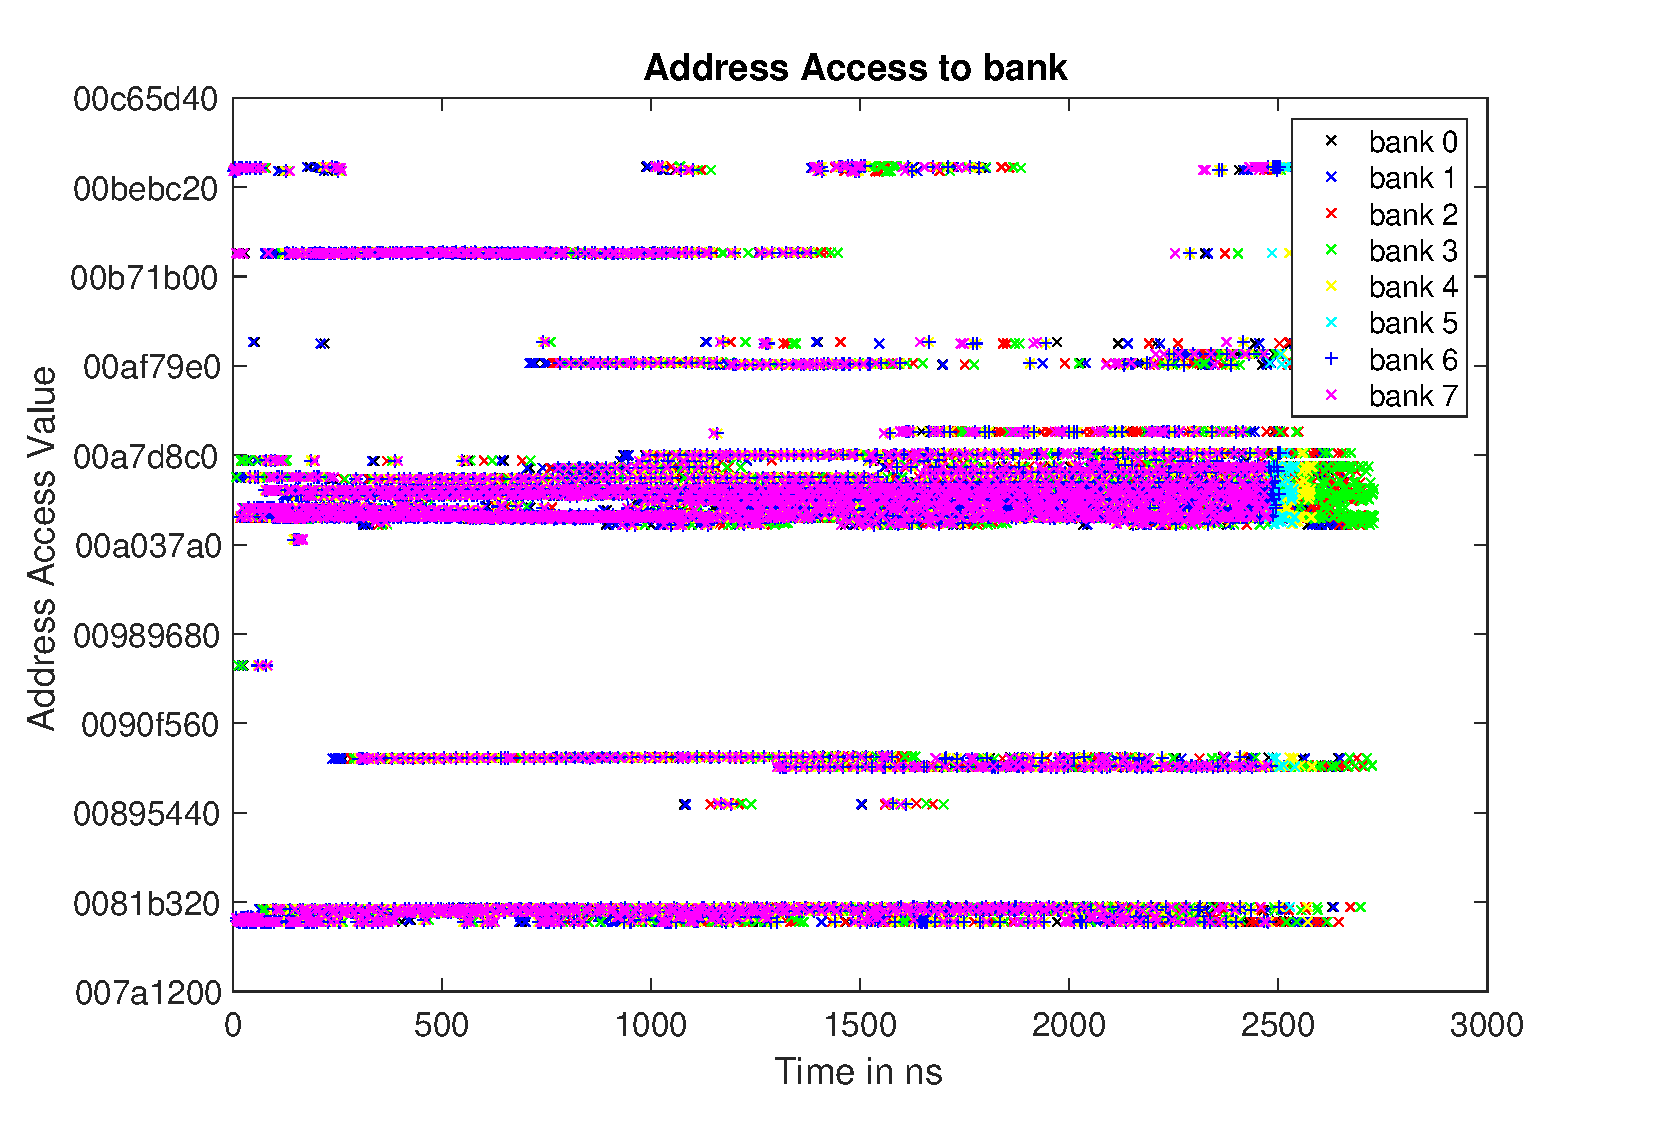
\includegraphics[width=0.50\linewidth]{figures/prefetch1.eps} 
%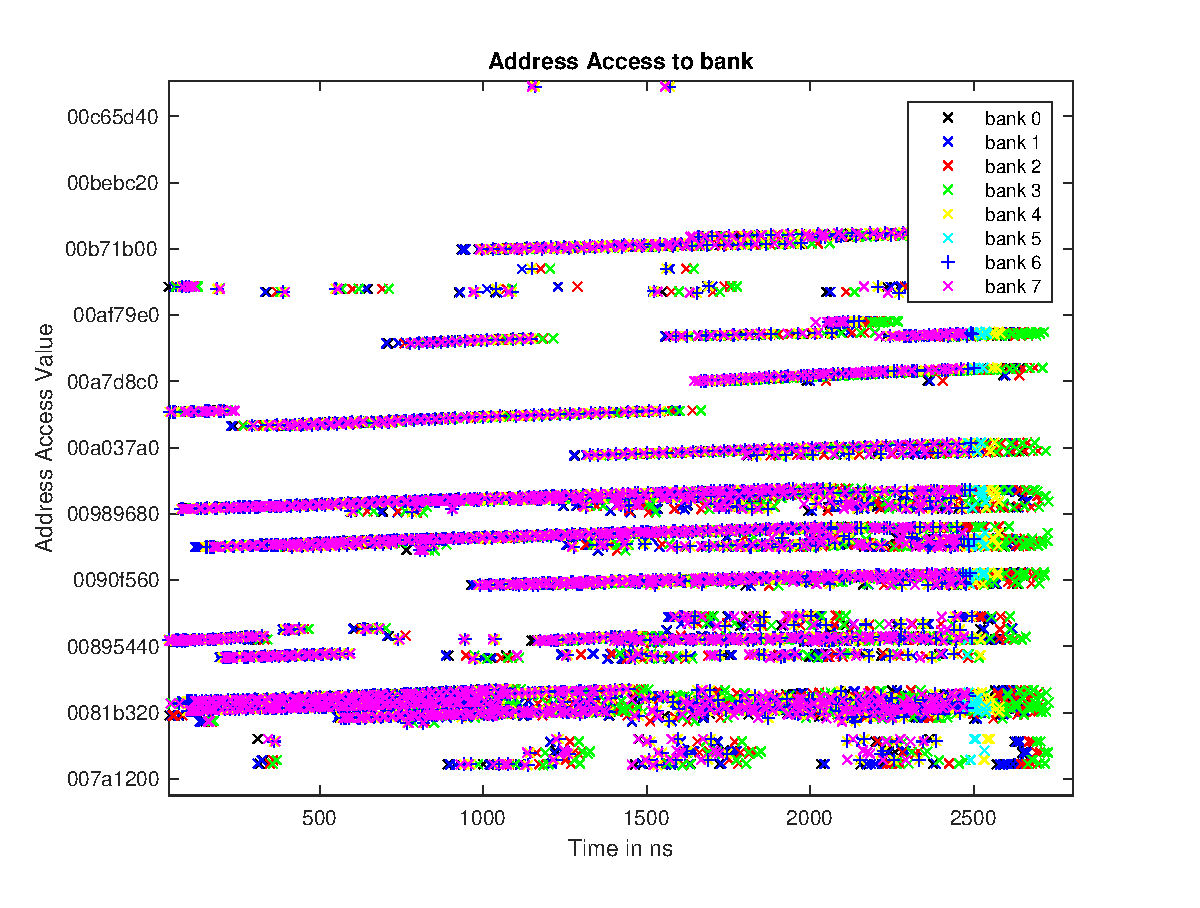
\includegraphics[width=0.46\linewidth]{figures/prefetch2.eps} 
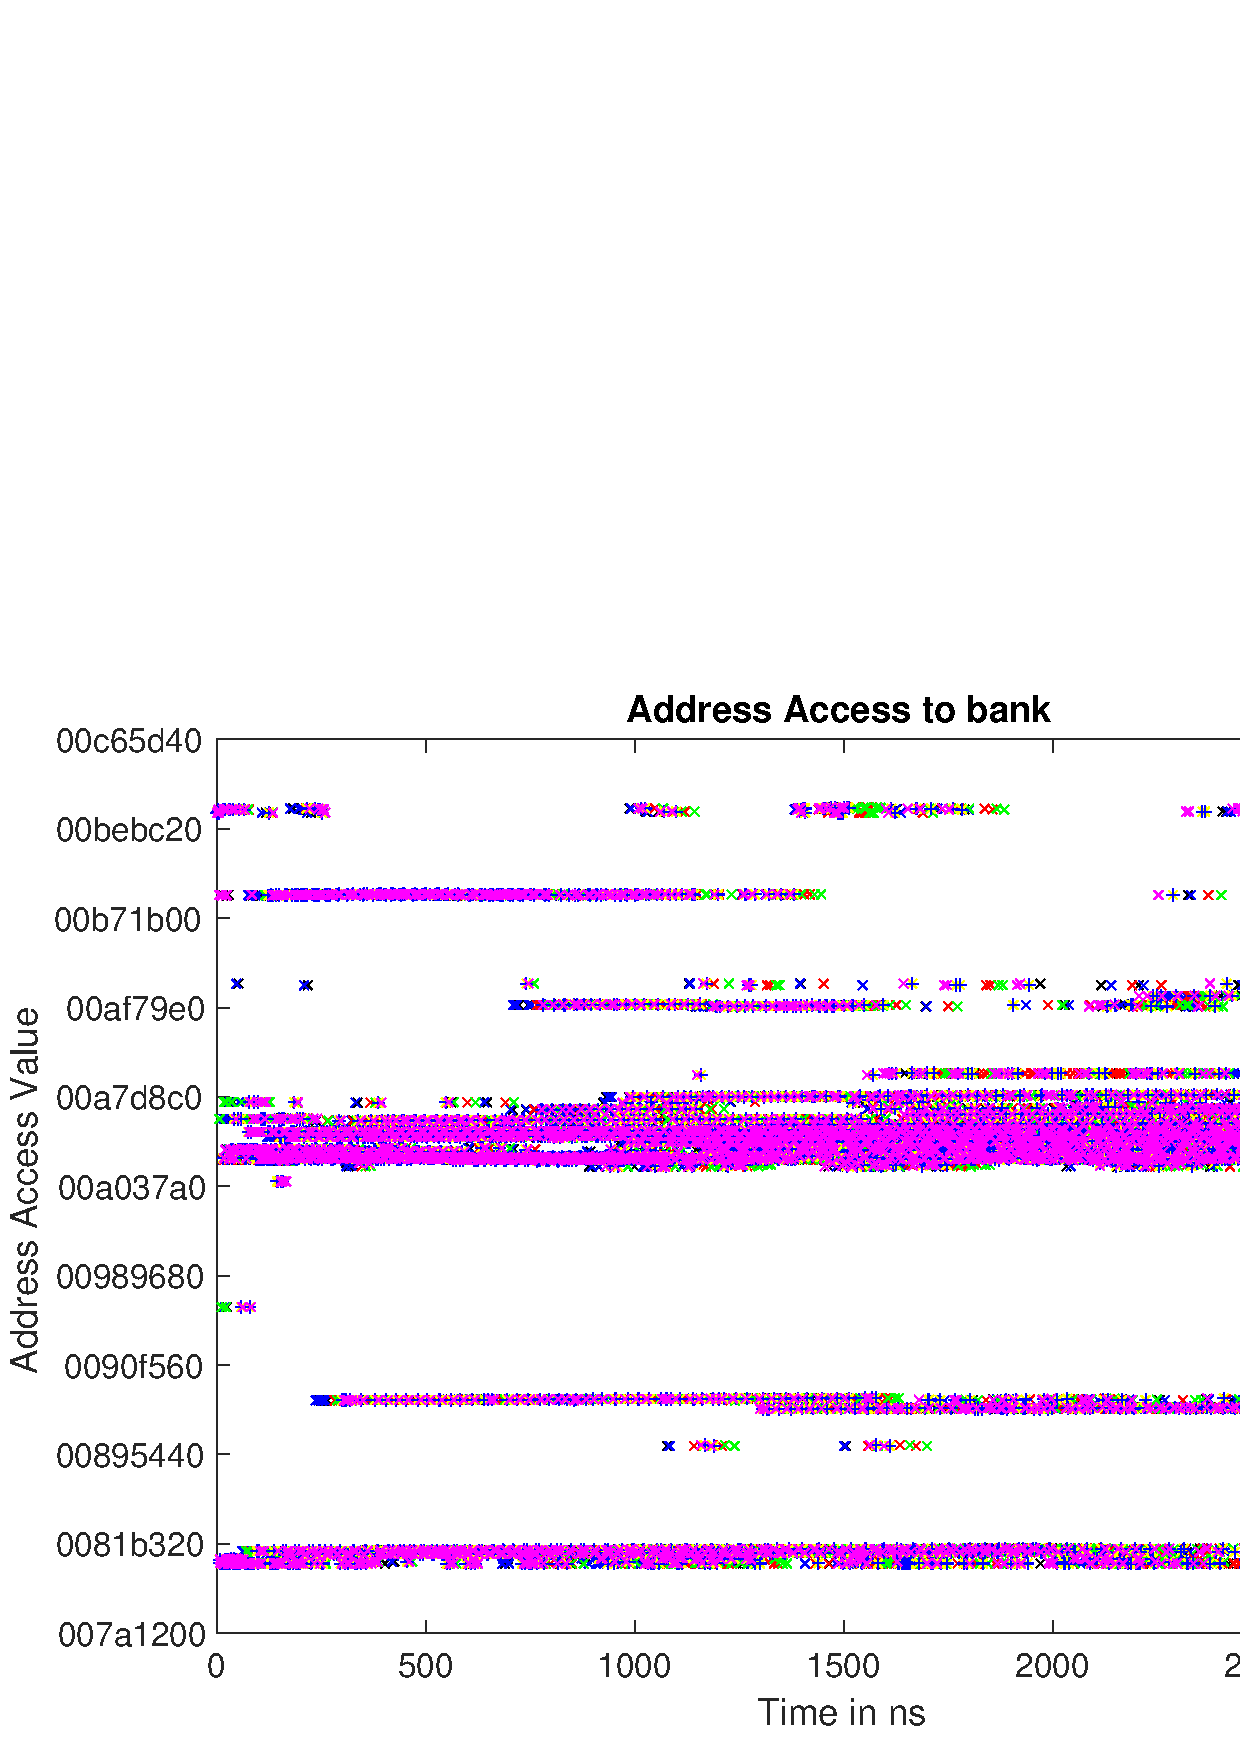
\includegraphics[width=3in,height=0.2\textheight]{figures/prefetch1.pdf}
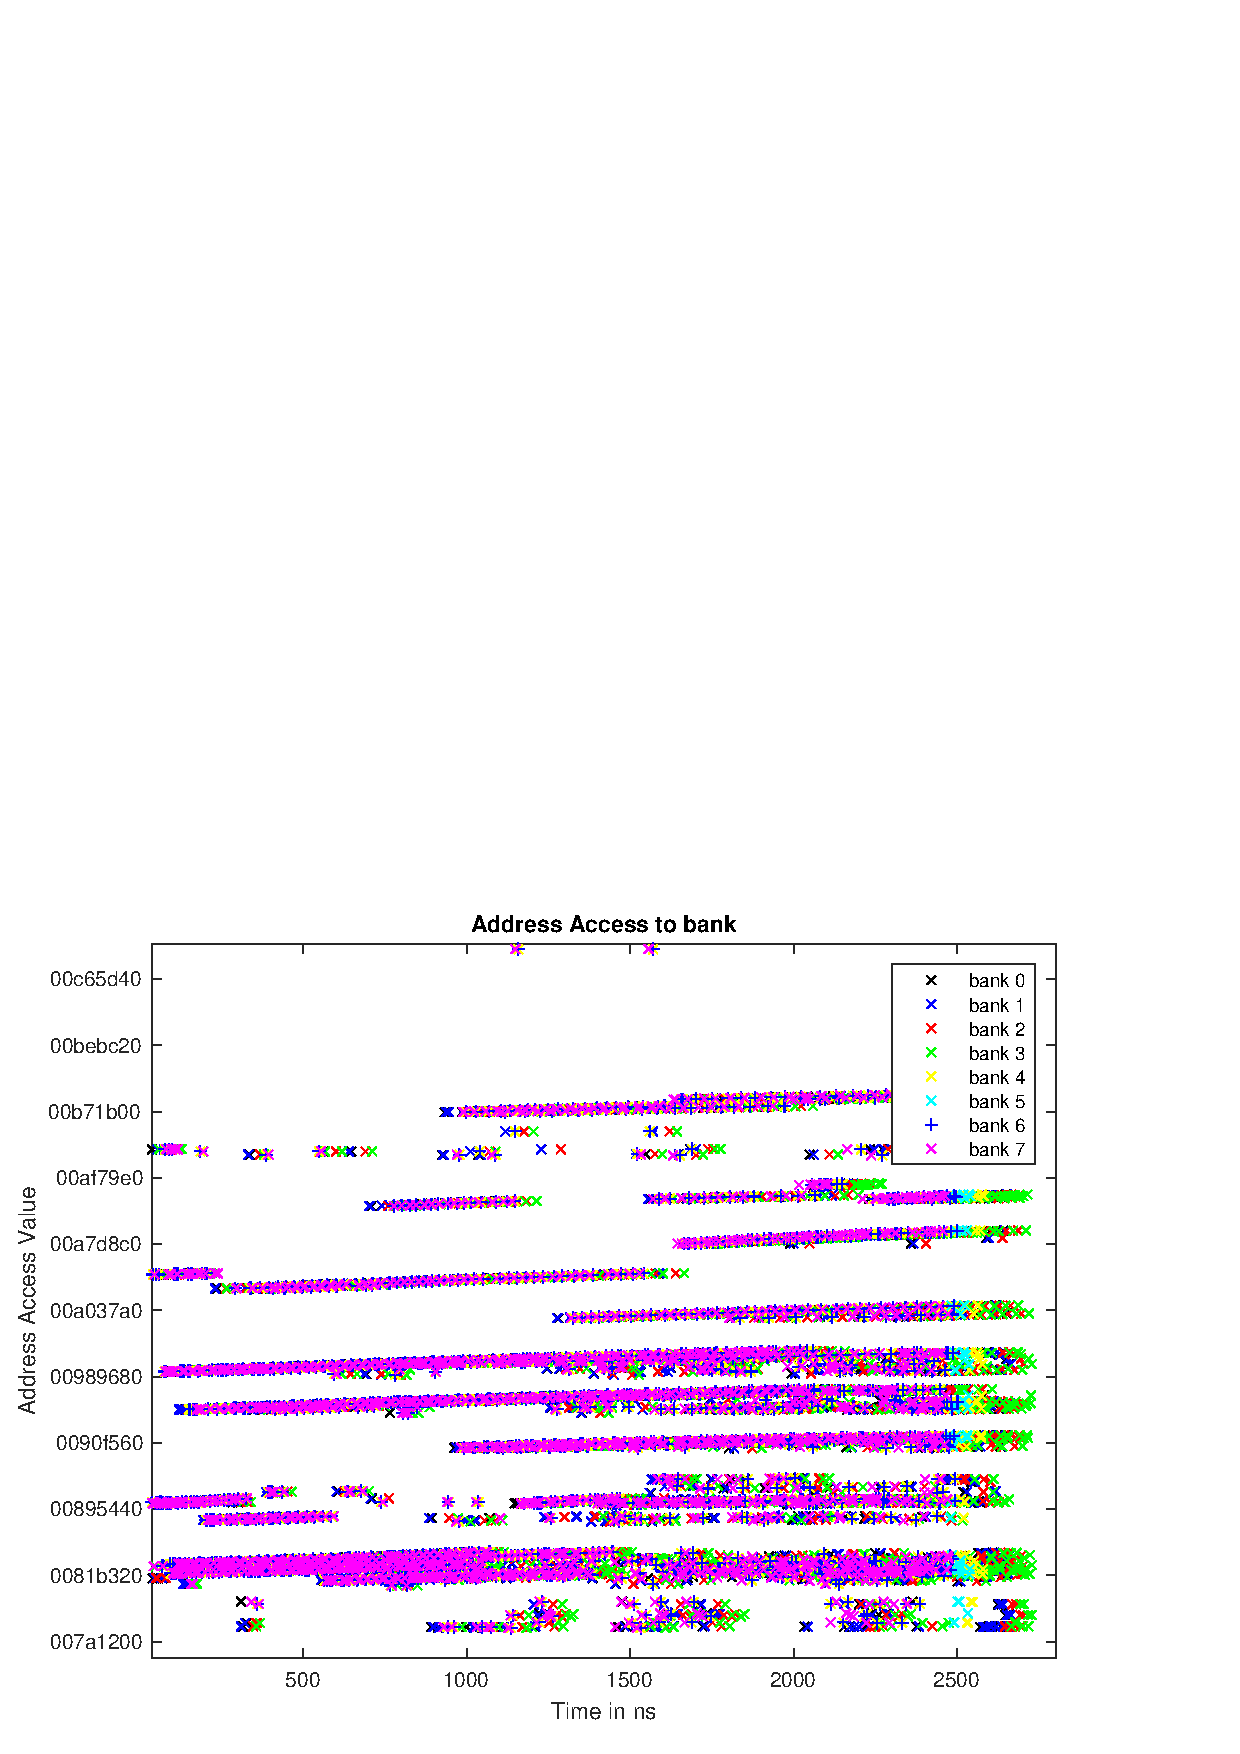
\includegraphics[width=2.6in,height=0.2\textheight]{figures/prefetch2.pdf}
\caption{Memory bank accesses across a 3 $\mu$s trace, which suggest linear access patterns. The right figure is an enlarged version of the top half of the left figure. }
\label{fig:prefetch1}
\end{figure*}
%%%%%%%%%%%%%%%%%%%%%%%%%%%%%%%%%%%

%{\color{blue} \noindent \textbf{Potential improvement using prefetching:}~
%\Ethan{Remove entire subsection?}
%We explore the implementation of a memory prefetching unit, similar to an instruction or cache prefetching unit. This unit can detect linear access patterns to regions in memory.  For example, if a string of memory accesses are issued in sequential byte sized order, then the prefetching unit will predict the next access to be in byte increments. The memory prefetching works by fetching a predicted address from the parity bank during accesses that the parity bank is idle. When future memory accesses are issued, they are first checked with the prefetched data to see if they can be used to decode any subsequent accesses memory accesses. If so, the memory access is obtained from the current accesses and prefetched data. 
%
%For example, say the prefetcher sees 2 consecutive memory requests in a row. It then predicts that the next two accesses, locations $a_0$ and $b_0$, are likely to be accessed in the near future. It reads $a_0 + b_0$ from the parity bank for future use. Next, access to location $a_0$ and $b_0$ are issued to the memory. Now, instead of reading both $a_0$ and $b_0$, only a single location has to be read from in memory, while the other location can be obtained from the prefetched data. This allows for an additional access to be issued from the now free memory bank.  In these cases, it is possible to obtain up to two additional memory accesses in a given cycle, one from the prefetched data and one from the parity bank.
%
%%Implementation of a memory prefetch should only require overhead for space and the associated logic to implement it. Since memory accesses are often stalled due to bank conflicts, checking pending accesses to the prefetched data should require no additional time overhead. As memory accesses wait to be issued in the bank queues, they can simultaneously be checked with the prefetched data. Thus, no extra latency is anticipated by the addition of a memory prefetching unit.
%
%Figure~\ref{fig:prefetch1} shows two plots of memory accesses to a bank with respect to time. The left figure shows the accesses to the memory bank by various cores. The right side figure shows a zoomed view of the accesses in the dense access region. This figure suggests the linearity of accesses. The system can look ahead in the queue to detect the consecutive address request for a memory bank and schedule a prefetch of the associated code.
%
%\noindent {\bf Coding and prefetching:~}One of the ideas explored in this paper is that of proactive prefetching of data from (unused) memory banks to buffers based on the pattern of pending access requests at the memory controller. This creates the opportunities to serve multiple access requests in a given memory cycles and also tries to utilize all the available memory banks throughout the operation of the memory system. Such prefetching based memory designs in the context of {\em uncoded} memory systems has been previously studied in the literature (see e.g.,~\cite{Kim2016, Kadjo2014, Shevgoor2015, JL2013}). To the best of our knowledge, the application of prefetching schemes with coded memory systems has not been explored before.}